\section{Analysis}
\label{sec:analysis}

Analyzing very large traces can take a long time.  While our custom
binary format enables efficient analysis, and our analysis techniques
are efficient, it can still take 4-8 hours to analyze a single set of
the 2007 traces.  In practice, we analyze the traces in parallel on a
small cluster of 4 core 2.4GhZ Opterons.  Our analysis typically
becomes bottle-necked on the fileservers that serve up to 200MB/s each
once an analysis is running on more than 20 machines.

We collected data at two times: 2003 (animation-2003), and 2007
(animation-2007).  During each time, we would start the collection
process, and let it run either until we ran out of disk space, or we
had collected all the data we wanted.  Each of these runs comprises a
set.  We have 21 sets from 2003, and 8 sets from 2007.

\subsection{Capture performance}

We start our analysis by looking at the performance of our capture
tool.  This validates our claims that we can capture packets at very
high data rates.  We examine the capture rate of the tool by
calculating the megabits/s (Mbps) and kilo-packets/s (kpps) for
overlapping intervals of a specified length.  For example if our
interval length is 60 seconds, then we will calculate the bandwidth
for the interval 0s-60s, 3s-63s, 6s-66s, ... end-of-trace.  We chose
to calculate the bandwidth for overlapping intervals so that if there
is any aligned cyclicality in the trace data we will not be confused
by it.  We divide an interval into 20 sub-intervals.  We then add the
interval's rate to an approximate quantile so that we can understand
the distribution of rates even for small intervals.  For example, we
have 11.6 billion measurements for animation-2007/set-0 at a 1ms interval
length.  This correspond to the 6.7 days of that trace.
% 11.6 * 10^9 * 0.001 / 20 = 580,000 / 86400 = 6.7

Figure~\ref{fig:bwrolling-mbps}(a) shows the cdf of bandwidth for the
2007 traces using 60 second intervals.  Two traces stand out set-5 and
set-4.  Set-4 was a trace of an NFS cache, rather than clients, and so
shows a much lower aggregate rate.  Set-5 was the trace of a different
set of clients working on a different movie, and hence shows a very
different distribution.  The graph shows the effectiveness of our
tracing technology on real workloads as it can capture 60s intervals
above 3Gbits (375MB/s).  Indeed these traces show the requirement for
high speed tracing as 5-20\% of the traces intervals have sustained
intervals above 1Gbit, which is above the rate at which
Leung~\cite{LeungUsenix08} noted their tracing tool started to drop
packets.  The 2003 traces have a distribution of shapes because they
were taken on a wider variety of places in the network, and are much
lower because our 2003 capture technology could not capture as much
data, so we traced fewer machines at a time.

Figure~\ref{fig:bwrolling-mbps}(b) shows animation-2007/set-5 at different
interval lengths.  This graph emphasizes how bursty the traffic was
during this trace. While 50\% of the intervals were above 500Mbits for
60s intervals, only 30\% of the intervals were above 500Mbits for 1ms
intervals.  This burstiness is expected given that
general Ethernet traffic and filesystem
traffic~\cite{Gribble98selfsimilar} has been shown to be
self-similar~\cite{Leland94selfsimilar}, which implies it is bursty.
It does make it clear that we need to look at short time intervals in
order to get an accurate view of the data.

Figure~\ref{fig:bwrolling-mbps}(c) shows the tail of the distributions for
the capture rates for two of the trace sets.  The relative similarity
between the Mbps and kpps graphs is simply because packet size
distributions are relatively constant.  The traces show the remarkably high
burstiness of the 2007 traces.  While 90\% of the 1ms intervals are
below 2Gbits, 0.1\% are above 6Gbits.  We expect we would have seen
slightly higher rates, but because of our configuration error for the
2007 capture tool, we could not capture above about 8Gbits.

\begin{figure*}
%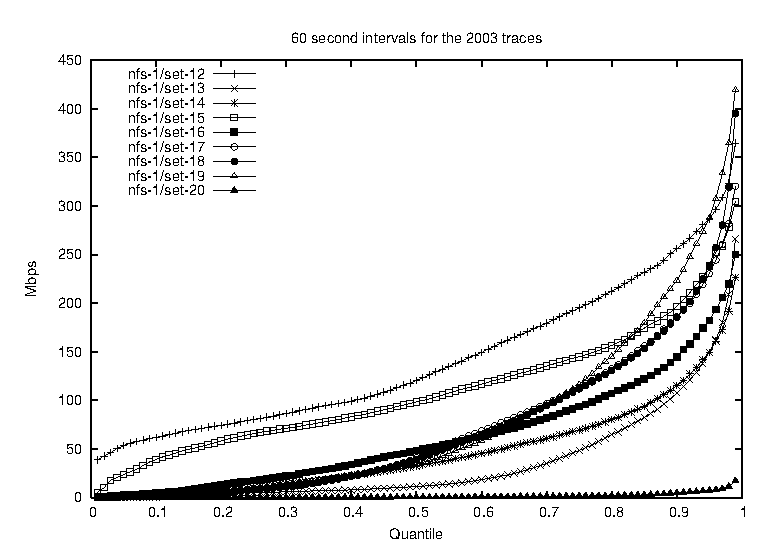
\epsfig{width=2.1in, angle=0, file=graphs/Mbps-nfs-1.ps}
%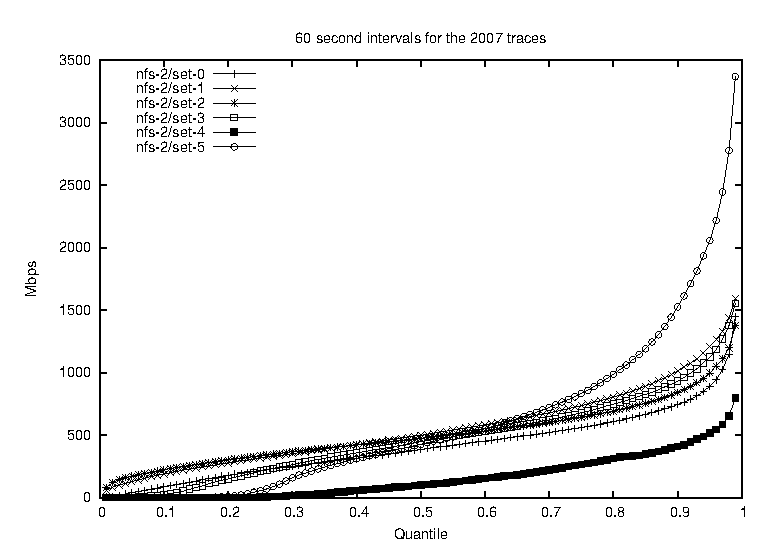
\epsfig{width=3.2in, angle=0, file=graphs/Mbps-nfs-2.ps}
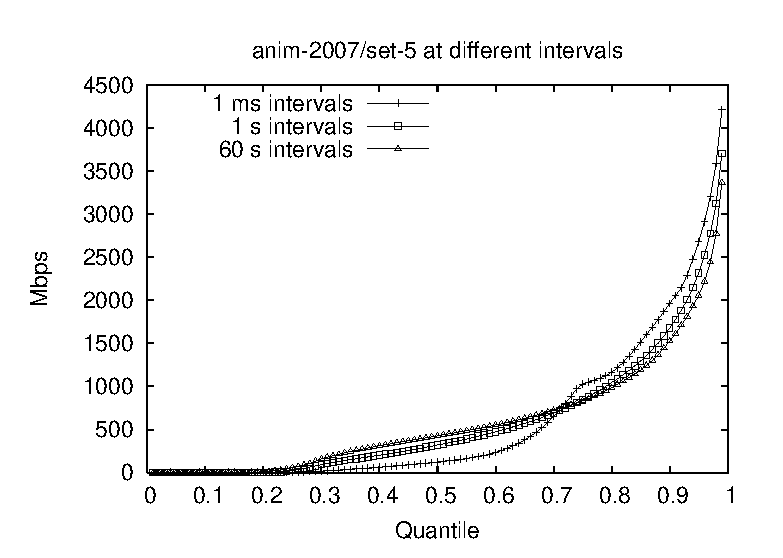
\epsfig{width=3.3in, angle=0, file=graphs/Mbps-nfs-2-set-5.ps}
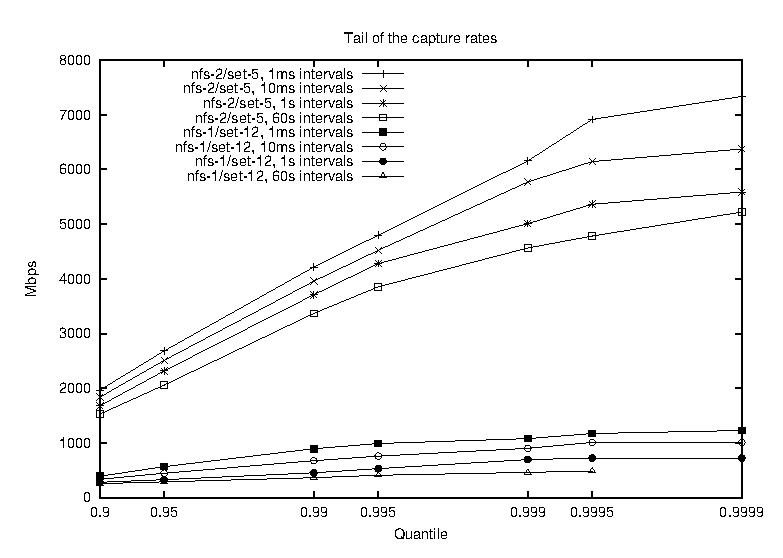
\epsfig{width=3.3in, angle=0, file=graphs/Mbps-tails.ps}
\caption{Bandwidth measured in the collection process.  In figure (b),
animation-2007/set-5 at different intervals is the top group of 4 lines, and
animation-2003/set-12 is the bottom group of 4 lines. animation-2003/set-12 does not go
all the way to the right at 60s intervals because there were
insufficient data points for the 0.9999 quantile.}
\label{fig:bwrolling-mbps}
\end{figure*}

% \begin{figure*}
% 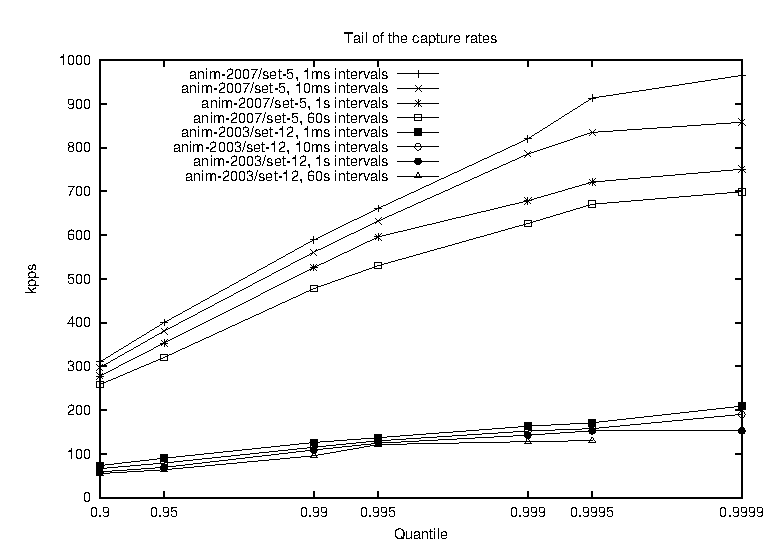
\epsfig{width=2.1in, angle=0, file=graphs/kpps-tails.ps}
% \caption{Tail of the quantiles in Mbps and kpps for the animation-2007 traces.}
% \label{fig:capture-tails}
% \end{figure*}

\subsection{Basic NFS analysis}

% nfs_hostinfo_rates, nfs_hostinfo_rate_quantiles, nfs_hostinfo_cube;
% choose sets nfs-2/set-[2,5]; nfs-1/set-[5,12]
%                     03+10, 06+13 ; 20+42, 27+49

% select from_unixtime(group_time), group_count/3600 where dataset = 'nfs-1/set-12' and group_time is not null and host is null  and operation is null and direction is null and op_dir is null
% nfs-1/set-5: 2003-09-16 .. 2003-09-18
% nfs-1/set-12: 2003-12-09 - 2003-12-10
% nfs-2/set-2: 2007-03-05 .. 2007-03-11
% nfs-2/set-5: 2007-10-12 .. 2007-10-17
% from hostinfo.hg + a few minor tweaks (n/a) for set-5 readdirplus
\begin{table*}
\begin{tabular}{|r||r|r||r|r||r|r||r|r|}
\hline
  & \multicolumn{2}{c||}{animation-2003/set-12} & \multicolumn{2}{c||}{animation-2003/set-5} & \multicolumn{2}{c||}{animation-2007/set-2} & \multicolumn{2}{c|}{animation-2007/set-5} \\
   operation &   Mops & bytes/op &   Mops & bytes/op &   Mops & bytes/op &   Mops & bytes/op \\
\hline
%     symlink &     0.008 &   201 &     0.000 &    92 &     0.001 &   415 &     0.000 &   458 \\
%       rmdir &     0.204 &   152 &     0.001 &    64 &     0.020 &   167 &     0.002 &   178 \\
%       mkdir &     0.173 &   304 &     0.005 &   193 &     0.071 &   336 &     0.004 &   334 \\
%      rename &     0.028 &   270 &     0.002 &   150 &     0.250 &   367 &     0.055 &   348 \\
%\hline
%      fsinfo &     0.023 &   176 &     0.003 &    72 &     1.352 &   176 &     0.619 &   176 \\
%        link &     0.000 &    86 &     0.000 &    88 &     3.259 &   314 &     0.182 &   322 \\
%        null &     0.259 &     5 &     0.087 &     4 &     1.482 &     4 &     2.808 &     4 \\
%      create &     0.296 &   295 &     0.965 &   200 &     4.639 &   367 &     1.616 &   344 \\
%\hline
%      remove &     0.275 &   136 &     0.641 &    69 &     8.419 &   194 &     1.500 &   186 \\
%     setattr &     0.716 &   133 &     1.075 &   136 &     9.415 &   193 &     6.531 &   192 \\
     readdir &     4.579 &   281 &     1.132 &  3940 &    28.318 &  4089 &    18.350 &  4071 \\
 readdirplus &     0.632 &  2307 &     0.000 &  n/a  &    32.806 &  1890 &    20.271 &  2001 \\
    readlink &     0.081 &    74 &     0.049 &    79 &    25.421 &   204 &    42.335 &   203 \\
      fsstat &    19.875 &    56 &    50.416 &    56 &     0.017 &   180 &     0.003 &   180 \\
       write &    14.546 &  9637 &    30.236 &  7880 &    32.390 & 13562 &    45.177 & 15015 \\
\hline
      lookup &   134.108 &    83 &    82.823 &    92 &   643.854 &   239 &   807.127 &   235 \\
        read &   345.743 &  1231 &   165.969 &  7855 &  1460.669 & 14658 &  1761.199 & 12301 \\
      access &     1.858 &   136 &     0.000 &   136 &  4000.204 &   136 &  3570.404 &   136 \\
     getattr &   244.650 &   104 &   967.961 &   104 &  6598.515 &   124 &  2756.785 &   123 \\
\hline
 {\bf total} &   768.053 &   790 &  1301.364 &  1274 & 12851.102 &  1833 &  9034.968 &  2599 \\
\hline
\end{tabular}

\caption{symlink, rmdir, mkdir, and rename were pruned as there were
fewer than 1 million operations; fsinfo, link, null, create, remove,
and setattr were pruned as there were fewer than 10 million
operations.  The Mops column could be calculated from nfsstat, but the
bytes/op column could not.}

\label{table:nfs-stats-overview}
\end{table*}

\begin{figure*}
% 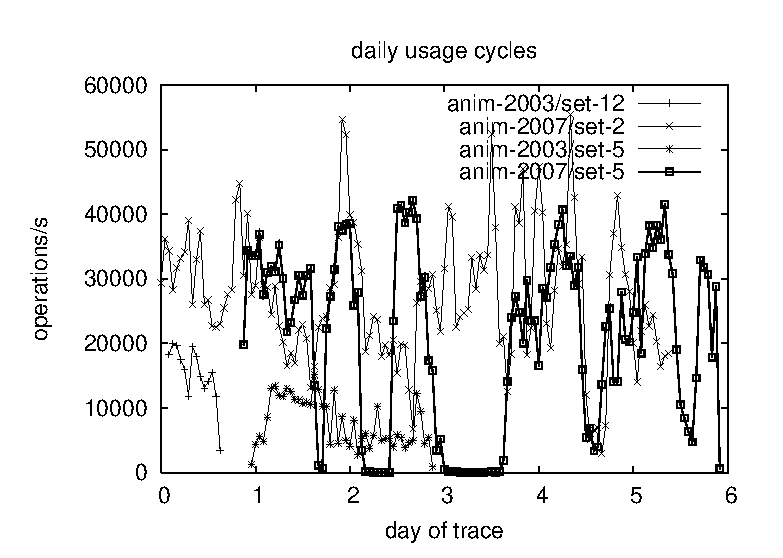
\epsfig{width=2.1in, angle=0, file=graphs/daily-oprate.ps}
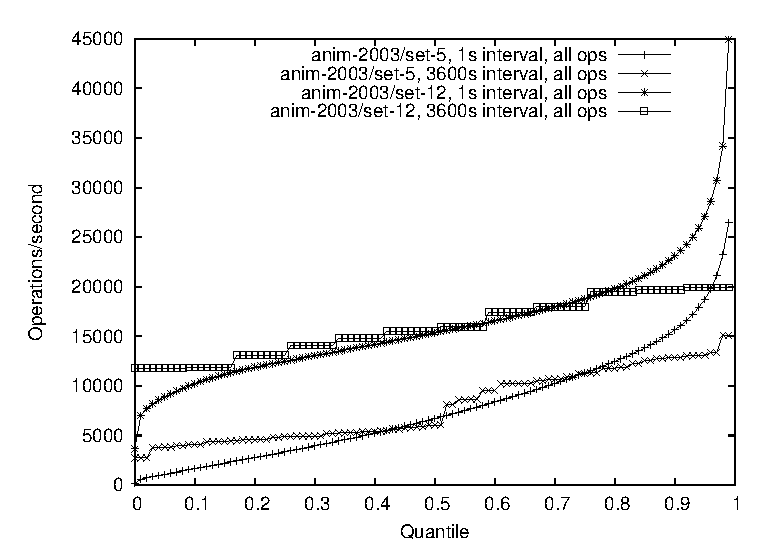
\epsfig{width=3.3in, angle=0, file=graphs/allops-quantile-nfs-1.ps}
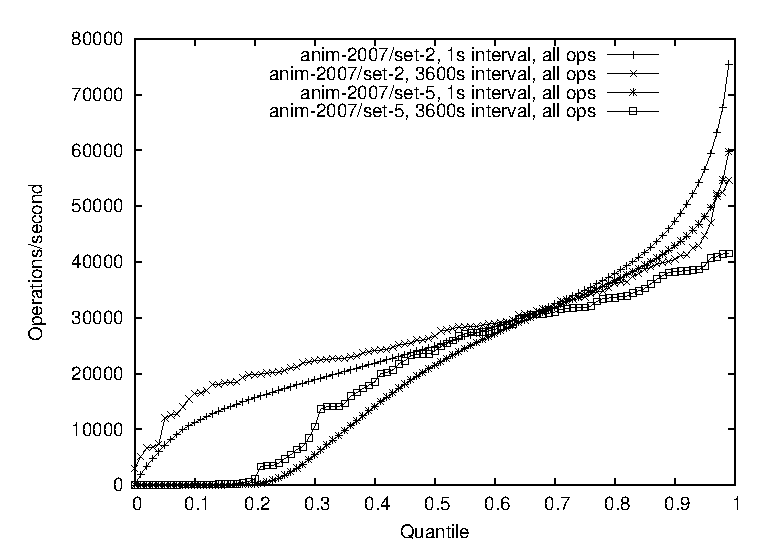
\epsfig{width=3.3in, angle=0, file=graphs/allops-quantile-nfs-2.ps}
\caption{Operation rates, as quantiles for anim-2003, anim-2007.}
\label{fig:oprates}
\end{figure*}

\begin{figure*}
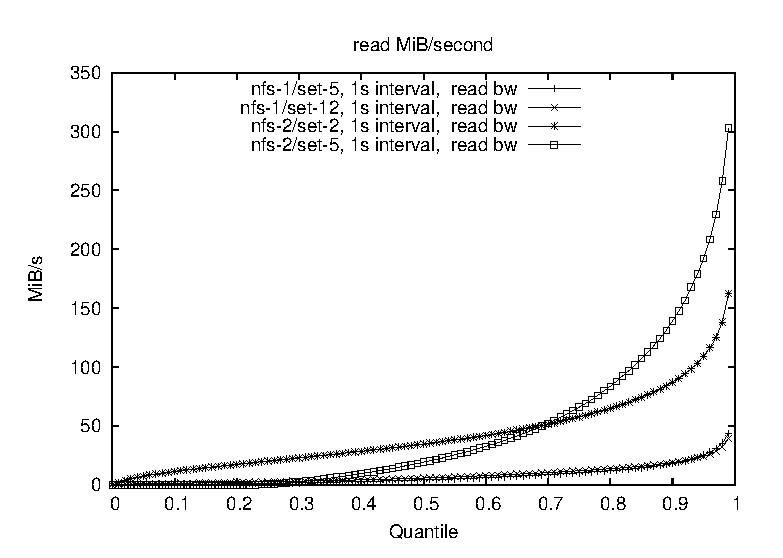
\epsfig{width=3.3in, angle=0, file=graphs/bw-read.ps}
%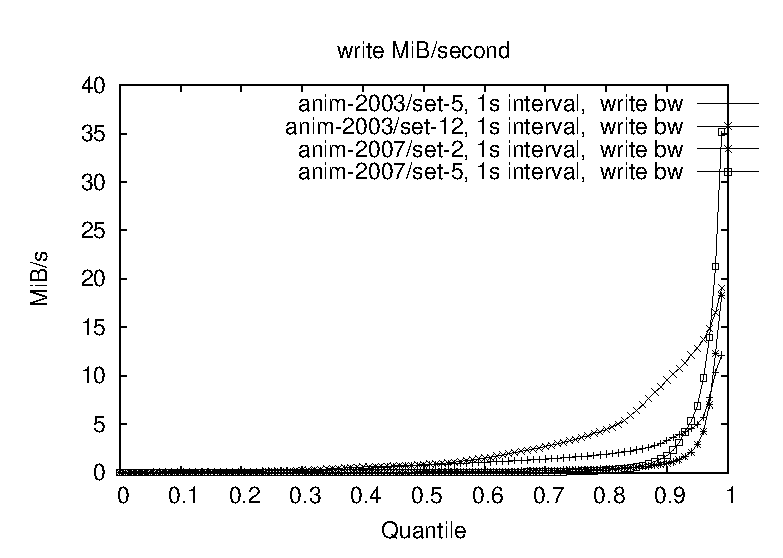
\epsfig{width=2.1in, angle=0, file=graphs/bw-write.ps}
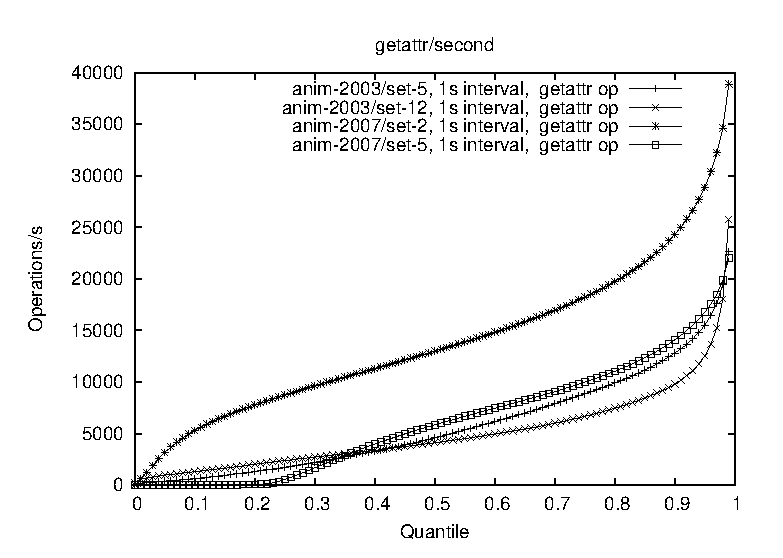
\epsfig{width=3.3in, angle=0, file=graphs/ops-getattr.ps}
\caption{Bandwidth for reads and operation rate for getattrs in the four traces.}
\label{fig:bw-ops-quantiles}
\end{figure*}

Examining the overall set of operations used by a workload provides
insight into what operations need to be optimized to support the
workload.  Examining the distribution of rates for the workload tells
us if the workload is bursty, and hence we need to handle a higher
rate than would be implied by mean arrival rates, and if there are
periods of idleness that could be exploited.

Table~\ref{table:nfs-stats-overview} provides an overview of all the
operations that occurred in the four traces we are examining in more
detail.  It shows a number of substantial changes in the workload
presented to the NFS subsystem.  First, the read and write sizes have
almost doubled from the animation-2003 to animation-2007 datasets.  This is expected
because the company moved from NFSv2 to NFSv3 between the two
tracing periods, and set the v3 read/write size to 16k.  We asked and
were told they set it to those sized based on some performance
measurements of sequential I/O.  The NFS version switch also accounts
for the increase in access calls (new in v3), and readdirplus (also
new in v3).  

We also see that this workload is incredibly read-heavy.  This is
expected; the animation workload reads a very large amount of
textures, models, etc. to produce a relatively small output frame.
However, we believe that our traces under-estimate the number of write
operations.  We discuss the write operation underestimation below.
The abnormally low read size for set-12 occurred because
that filer was handling a large number of stale FH requests.  The
replies were therefore small and pulled down the bytes/operation.  We
see a lot more getattr operations in set-5 than set-12 because set-12
is a filer behind some nfs-caches, whereas set-5 is the workload
before the nfs-caches.

Table~\ref{table:99quant-differences} and
figure~\ref{fig:oprates}(b,c) shows how long averaging intervals
can distort the load placed on the storage system.  If we were to
develop a storage system for the hourly loads reported in most papers,
we would fail to support the substantially higher near peak (99\%)
loads seen in the data.  It also hides periods of idleness
that could be used for incremental scrubbing and data reorganization.

We include figure~\ref{fig:oprates}(a) because it is the traditional
graph that shows daily cycles.  We do not have quite as strong daily
cycles because animation companies are good at keeping their compute
clusters busy overnight, but we can see for animation-2007/set-5 the effect of
the weekends where the load on the system drops nearly to 0.

Figure~\ref{fig:bw-ops-quantiles} shows the read and write MiB/s and the
getattr operations/s.  It shows that relative to the amount of data
being transferred, the number of getattrs has been reduced, likely a
result of the transition from NFSv2 to NFSv3.  The graph shows the
payload data transferred, so it includes the offset and filehandle of
the read request, and the size and data in the reply, but does not
include IP headers or NFS RPC headers.  It shows that the NFS system
is driven heavily, but not excessively, and it seems to imply that the
write bandwidth has gotten more bursty, but has stayed roughly
constant.  

This result led us to further analyze the data.  We were surprised
that that write bandwidth would not increase, even though it is not
implausible as the frame output size has not increased.  We analyzed
the traces to look for missing operations in the sequence of
transaction ids, automatically inferring if the client is using a
big-endian or little-endian counter.  The initial results looked quite
good, animation-2007/set-2 showed 99.7\% of the operations were in sequence,
animation-2007/set-5 showed 98.4\%, and counting the skips of 128 transactions
or less, we found only 0.21\% and 0.50\% respectively (the remaining
entries were duplicates or ones that we could not positively tell if
they were in sequence or a skip).  However, when we looked one level
deeper at the operation that preceded a skip in the sequence, we found
that 95\% of the skips followed a write operation for set-2, and 45\%
for set-5.  The skips in set-2 could increase the write workload by a
factor of 1.5x if all missing skips after writes are associated with
writes.  We expected a fair number of skips for set-5 since we
experienced packet loss under load, but we did not expect it for
set-2.

Further examination indicated that the problem came about because we
followed the same parsing technique for TCP packets as was used in
nfsdump2~\cite{ellardTraces}.  We started at the beginning of the
packet and parsed all of the RPCs that we found that matched all
required bits to be RPCs.  Unfortunately, over TCP, two back to back
writes will not align the second write RPC with the packet header, and
we will miss subsequent operations until they re-align with the packet
start.  While the fraction of missing operations is small, they are
biased toward writes (read replies can only be affected if the second
read reply is close enough to the first that they are combined).  This
leads us to one of our lessons, extensive validation of the conversion
tool is important.  Both validation through validation statistics, and
through the use of a known workload that exercises the capture tools.
An NFS replay tool~\cite{NingningFast05} could be used to validate
that the captured workload is the one that was replayed.  This
comparison has been done to validate a block based replay
tool~\cite{AndersonFast04}, but has not been done to validate a
capture tool, as that work simply assumed capture was correct.
\fix{create analysis that compares timing of ops to packets and
estimates missing writes if we can get the space for it} 
% We can therefore use
% the timing information from requests and replies to identify gaps in
% the dataset and determine how many bytes were skipped.  This will
% allow us to approximate the number of missing writes.  Preservation of
% lower level information is a lesson we got right, and it will allow us
% to partially reconstruct flaws in the traces.  
We believe a similar
flaw is present in earlier traces~\cite{ellardTraces} because the same
parsing technique was used, we do not know how much those traces were
affected.

% select dataset, group_seconds, operations_per_second from xnfs_hostinfo_rate_quantiles where host is null and direction = 'send' and operation is null and op_dir is null and quantile = 0.99
\begin{table}
\begin{tabular}{|l|r|r|r|}
\hline
dataset & 1s ops/s & 3600s ops/s & ratio \\
\hline
anim-2003/set-5  & 26,445 & 15,110 & 1.75x \\
anim-2003/set-12 & 44,926 & 19,923 & 2.25x \\
anim-2007/set-2  & 75,457 & 54,657 & 1.38x \\
anim-2007/set-5  & 59,727 & 41,550 & 1.44x \\
\hline
\end{tabular}
\caption{Ratio between operation rates at 1 second and one hour grouping sizes}
\label{table:99quant-differences}
\end{table}

\subsection{File sizes}

\begin{figure}
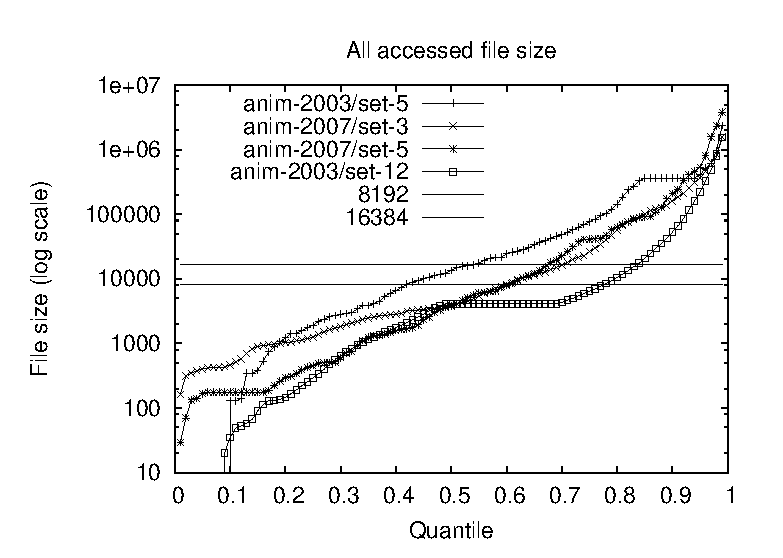
\epsfig{width=3.2in, angle=0, file=graphs/file-size.ps}
\caption{File size distribution for all accessed files.}
\label{fig:file-size}
\end{figure}

File sizes affect the potential internal fragmentation for a
filesystem.  They affect the maximum size of I/Os that could be
executed, and they affect the potential sequentiality in a workload.

Figure~\ref{fig:file-size} shows the size of files accessed in our
traces.  It shows that the files in the animation workload are in
general very small, as 40-80\% of the files are smaller than 8k, and
hence will be read in a single I/O for the 2003 traces.  70\% of the
files are smaller than 16k for the 2007 traces, and hence will be read
in a single I/O.  While there are larger files in the traces, 99\% of
the files are smaller than 10MB.  The small file sizes present in this
workload, and the preponderance of writes suggest that a flash file
system~\cite{Kawaguchi95aflash-memory} or MEMS file
system~\cite{SchlosserFast04} could support a substantial portion of
the workload.

\subsection{Sequentiality}

\begin{figure*}
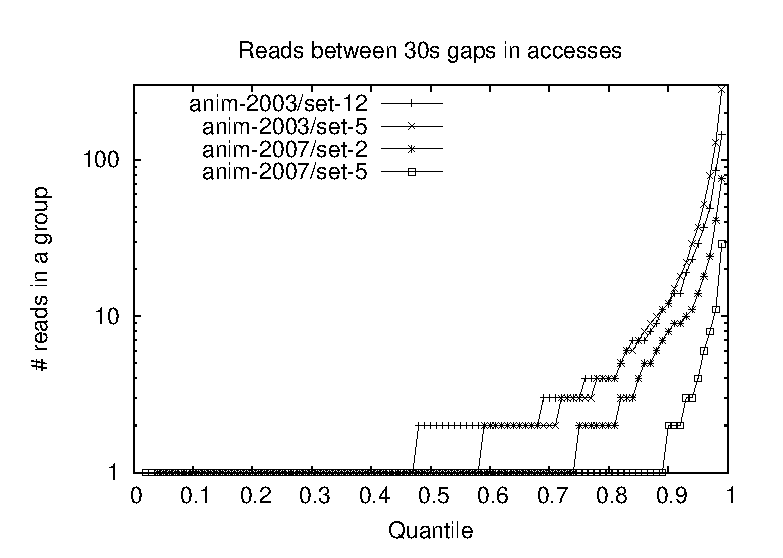
\epsfig{width=3.3in, angle=0, file=graphs/seq-read-group-counts.ps}
% 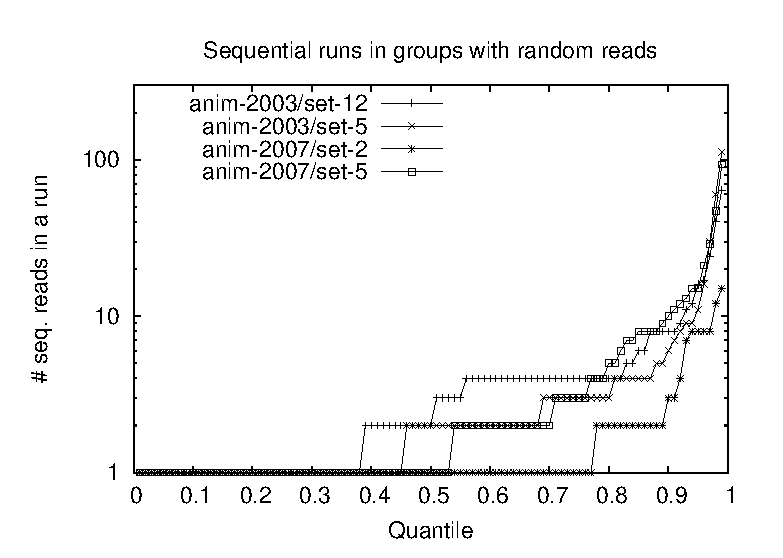
\epsfig{width=2.1in, angle=0, file=graphs/seq-in-random-seq-count.ps}
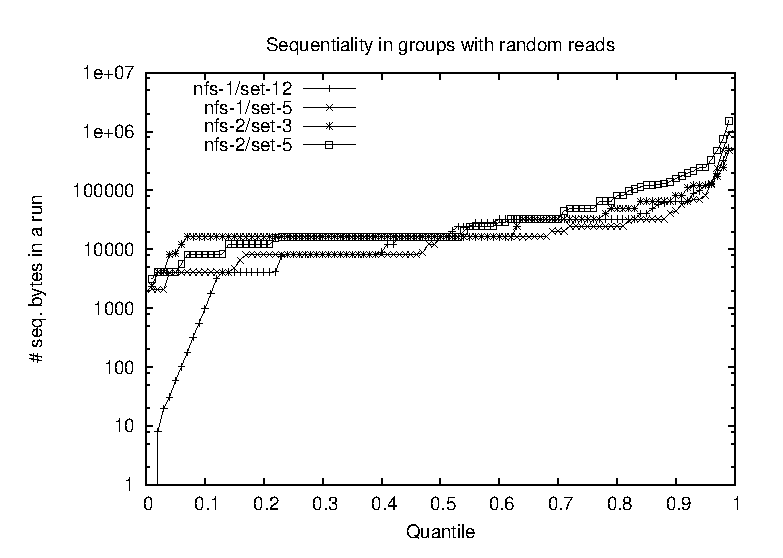
\epsfig{width=3.3in, angle=0, file=graphs/seq-in-random-seq-bytes.ps}
\caption{number of reads in a single group (more than 30s gap between I/Os); }
\label{fig:seq-analysis}
\end{figure*}

\begin{figure}
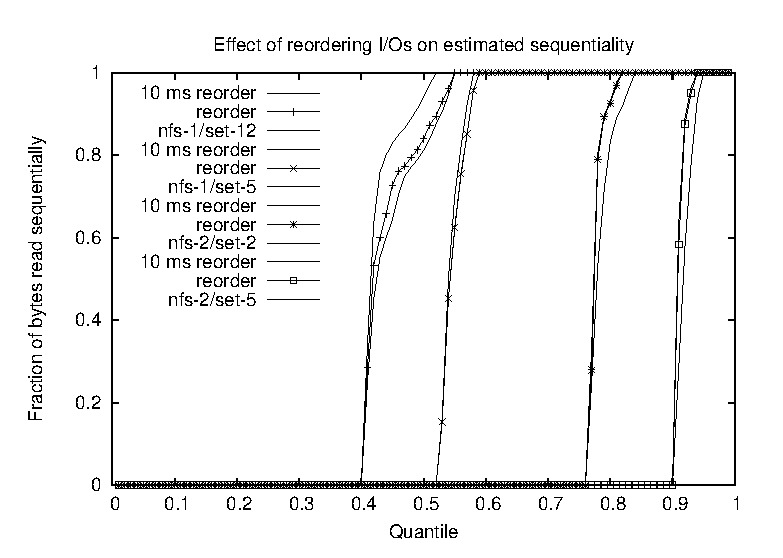
\epsfig{width=3.2in, angle=0, file=graphs/seq-bytes-compare.ps}
\caption{Negligible effect of reordering I/Os to improve estimated sequentiality.}
\label{fig:seq-bytes-compare}
\end{figure}

Sequentiality is one of the most important properties for storage
systems because disks are much more efficient when handling sequential
data rather than random accesses.  Prior work has presented
various methods for calculating sequentiality.  Both
Ellard~\cite{EllardFast03} and Leung~\cite{LeungUsenix08} split accesses
into groups and calculate the sequentiality within the group.  Ellard
emulates opens and closes by looking for 30s groups in the access
pattern.  Ellard tolerates small gaps in the request stream as
sequential, e.g. an I/O of 7k at offset 0 followed by an I/O of 8k at
offset 8k would be considered sequential.  Ellard also re-orders I/Os
to deal with client-side reordering. In particular Ellard looks
forward a constant amount from the request time to find I/Os that
could make the access pattern more sequential.  This constant was
determined empirically.  Leung treats the first I/O after an open as
sequential.

We prefer to only reorder within overlapping requests. Given two I/Os,
A, and B, if the request-reply intervals overlap, then we are willing
to re-order the requests to improve estimated sequentiality.  We
believe this is a better model because the NFS server could have a
change to re-order those I/Os.  In practice
figure~\ref{fig:seq-bytes-compare} shows that for our traces this
reordering makes little difference.  Allowing reordering an additional
10ms beyond the reply of I/O A slightly increases the sequentiality,
but generally not much more than just for overlapping requests.

We also decide on whether the first I/O is sequential or random based
on additional I/Os.  If the second I/O (after any reordering) is
sequential to the first one, than the first I/O is sequential,
otherwise it is random.  If there is only one I/O to a particular
file, then we consider the I/O to be random since the NFS server would
have to reposition to that file to start the read.  

Given our small file sizes, it turns out that most accesses count as
random because they read the entire file in a single I/O.  We can see
this in figure~\ref{fig:seq-analysis}(a) which shows the number of
reads in a group.  Most groups are single I/O groups (70-90\% in the
2007 traces).  We see about twice as many I/Os in the 2003 traces,
because the I/Os in the 2003 traces are only 8KiB rather than 16KiB.

Sequential runs within a random group turns out to be more
interesting.  Figure~\ref{fig:seq-analysis}(b,c) show the number of
I/Os and the number of bytes accessed in sequential runs within a
random group.  We can see that if we start accessing a file at random,
most (50-80\%) of the time we will do single or double I/O accesses.
However we can also see that we can get some extended runs within a
random group, although 99\% of the runs are less than 1MB.

% select dataset,operation, max(mean_operations_per_second) from xnfs_hostinfo_rates where group_seconds = 1 and host is null and direction = 'send' and operation is not null and op_dir is null and mean_operations_per_second > 300 group by dataset,operation order by operation
% --> access, fsstat, getattr, lookup, read, write 

\fix{5. Cram another analysis in here: file size distribution by
access, or stack-distance}

